\section{Modelos de Neurônios}\label{section_modelos_neuronios} 

Em 1907, Lapicque desenvolveu um modelo de neurônio que descreve o neurônio como um circuito elétrico contendo um capacitor e um
resistor em paralelo, como representado na figura~\ref{fig_lapicque}, representando a capacitância e a resistência de vazamento da
membrana celular~\cite{lapicqueRecherches1907}, chamado de modelo Integrate-and-Fire (IF). Mesmo sem entender os mecanismos por
trás da geração de potenciais de ação, Lapicque postulou que, ao atingir um certo potencial limiar, um potencial de ação seria
gerado e o capacitor descarregado, reiniciando o potencial da membrana. Isso mostra que, ao se tratar de modelagem de neurônios,
estudos da função não necessariamente requerem conhecimento do mecanismo~\cite{abbottLapicque1999}. O modelo de neurônio de
Lapicque foi a primeira tentativa de representar matematicamente um neurônio biológico.

\begin{figure}[!ht]
\Caption{\label{fig_lapicque} (A) O circuito elétrico de Lapicque: I é a corrente injetada, C a capacitância da membrana, R a resistência da membrana,
V o potencial de membrana e $V_{rest}$ o potencial de repouso. (B) A trajetória de tensão, quando um limiar é atingido, um
potencial de ação é disparado. (C) Um modelo IF com corrente que varia pelo tempo.}
\centering
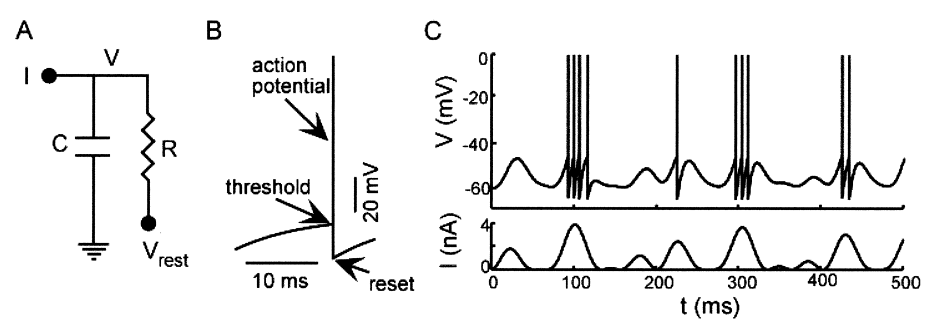
\includegraphics[width=\linewidth]{figuras/lapicque.png}
\Fonte{\cite{abbottLapicque1999}}
\end{figure}

O modelo de Hodgkin-Huxley~\cite{hodgkinQuantitative1952}, representou um avanço significativo na compreensão e na modelagem dos
neurônios biológicos. Diferentemente do primeiro modelo criado por Lapicque, esse modelo buscou descrever a geração e propagação
de potenciais de ação em neurônios levando em consideração os processos eletroquímicos subjacentes, como a dinâmica dos diferentes
canais iônicos que controlam a corrente elétrica através da membrana celular.

O modelo de Hodgkin-Huxley é composto por um conjunto de equações diferenciais ordinárias que descrevem a variação do potencial de
membrana em função do tempo e das correntes iônicas. Essas equações consideram o comportamento dinâmico dos canais iônicos de
sódio e potássio, bem como a corrente de vazamento através da membrana. O modelo é capaz de capturar o comportamento típico dos
neurônios, incluindo a resposta ao estímulo, a fase refratária e a propagação do sinal ao longo do axônio.

Baseados na ideia de Lapicque, hoje em dia são utilizados os modelos IF.\@Existem diversos modelos IF, com
várias modificações da ideia original, como o modelo Leaky Integrate-and-Fire (LIF)~\cite{burkittReview2006}. Os modelos IF são
uma alternativa mais simples e computacionalmente eficiente em comparação ao modelo de Hodgkin-Huxley. Embora não sejam tão
biologicamente precisos quanto o modelo de Hodgkin-Huxley, os modelos IF conseguem capturar algumas das características essenciais
dos neurônios, como a integração temporal dos estímulos e a emissão de potenciais de ação quando um limiar é atingido. Outra
vantagem dos modelos IF é que modelos simples são uma forma de reduzir a complexidade do cérebro para seus mecanismos mais
fundamentais.

Apesar de sua simplicidade, os modelos IF têm sido amplamente utilizados em RND devido à sua eficiência computacional e capacidade
de reproduzir aspectos fundamentais do comportamento neuronal. Por exemplo, no trabalho de~\cite{teeterGeneralized2018} o
comportamento de 645 neurônios do neocórtex foi reproduzido utilizando modelos GLIF (Generalized Leaky Integrate-and-Fire). 

O modelo de neurônio LIF é descrito pela dinâmica do potencial de membrana do neurônio, $v(t)$, que é dado pela
equação~\ref{eq_lif}

\begin{equation}
\label{eq_lif}
C_m \frac{dv(t)}{dt} = -\frac{C_m}{\tau_m} [v(t) - V_0] + I(t)
\end{equation}

onde $C_m$ é a capacitância da membrana, $V_0$ é o potencial de repouso, $\tau_m$ é a constante de tempo passiva da membrana
(relacionada à capacitância do neurônio e à resistência de vazamento do potencial de membrana por $\tau_m = R_m C_m$), $I(t)$ é a
corrente elétrica injetada no neurônio (tanto a corrente causada pelas sinapses, como a por eletrodos)~\cite{burkittReview2006}. 

Quando o potencial de membrana atinge um limiar, $V_{th}$, um potencial de ação é disparado e o potencial de membrana é resetado
para $V_{reset}$, o potencial um pouco menor que o potencial de repouso, correspondente ao período refratário do neurônio.

Existem diversos outros modelos de neurônios, como o modelo de Izhikevich~\cite{izhikevichSimple2003}, que é quase tão simples em
termos computacionais quanto o modelo IF, mas que consegue capturar de forma muito mais realista um conjunto maior de
comportamentos neurais dependendo dos parâmetros utilizados. Esse modelo é especialmente útil para simular neurônios específicos
do cérebro, enquanto os modelos IF são preferidos quando o objetivo é estudar o comportamento geral de neurônios por sua
simplicidade, e, portanto, serão utilizados nesse trabalho.

\begin{figure}[!ht]
\Caption{Diferentes tipos de neurônios simulados pelo modelo de Izhikevich.}
\centering\label{fig_izhikevich}
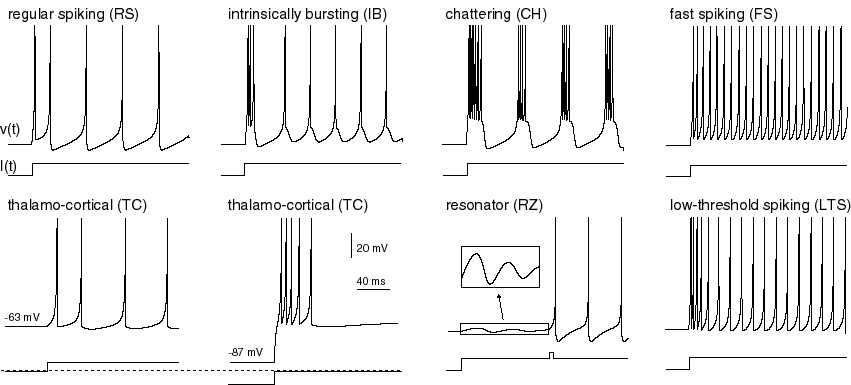
\includegraphics[width=\linewidth]{figuras/izhikevich.png}
\Fonte{\cite{izhikevichSimple2003}}
\end{figure}

\subsection{Modelos de Sinapses}\label{subsection_modelos_sinapses}

\begin{equation}
\label{eq_sinapse}
\frac{dg_{syn}(t)}{dt} = \bar{g}_{syn}\sum_{k}{\delta(t-t_k)} - g_{syn}(t)/\tau_{syn}
\end{equation}
